\section{Scheduling retraining and inference jointly}
\label{sec:motivation}
% This section motivates the scheduler

%Our goal is to utilize continuous learning (\S\ref{subsec:continuous}, \S\ref{subsec:continuous-measurement}) to maximize edge DNN accuracy in the face of data drift. 
%As continuous learning is a promising approach for data shift, we 
We propose \emph{joint retraining and inference} on edge servers.
The joint approach utilizes resources better than statically provisioning compute for retraining. Since retraining is periodic \cite{distribution-20, mullapudi2019} with far higher compute demands than inference, static provisioning causes idling.  
Compared to uploading videos to the cloud for retraining, our approach has advantages in privacy (\S\ref{subsec:edge}), and network costs and accuracy (\S\ref{subsec:eval-alternate}).
%Our approach also ensures everything is completed on the edge, which has clear advantages in network costs and privacy (\S\ref{subsec:edge}) over transmitting the videos to the cloud for retraining. 
%Our proposal is to extend the edge servers, which already performs video DNN inferences, to {\em include continuous training of the edge DNN models}. Edge servers have the capacity to store the limited amount of recent video data that is required for continuous retraining. However, the edge server's compute is already provisioned for the DNN inference on live video streams. %Since retraining is periodic, i.e., its compute requirements are bursty in nature, provisioning compute resources for retraining will lead to wasted utilization and increased cost (by as much as \gaa{XXX} in our experiments). 
%Statically provisioning additional resources for retraining is wasteful since retraining is periodic \cite{distribution-20, mullapudi2019} %\ion{Cite something to support the statement that retraining is periodic} 
%Uploading videos to the cloud for retraining 
%For the reasons explained in \S\ref{subsec:edge} -- bandwidth constraints and privacy sensitivities -- transmitting the videos to the cloud for retraining is not preferred. In fact, our analysis in \S\ref{subsec:eval-alternate} shows that sending data to the cloud for retraining adds significant delays due to network overheads.

%We present the properties of the configurations for continuous training and inference on the DNNs (\S\ref{subsec:profiles}), and describe an example to motivate their joint scheduling (\S\ref{subsec:motivation-sched-example}).

%Joint retraining and inference involves complex trade-offs among retraining and inference jobs for many video streams. \S\ref{subsec:profiles} describes the tradeoffs in retraining and inference configurations, and \S\ref{subsec:motivation-sched-example} presents an example to illustrate the tradeoffs in configuration selection and resource allocation. %uses an example to illustrate the scheduling considerations in configuration selection and resource allocation. 

\begin{figure}[t]
  \centering
   \begin{subfigure}[t]{0.47\linewidth}
    \centering
    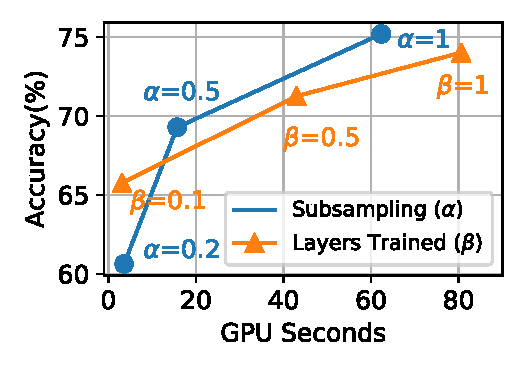
\includegraphics[width=\linewidth]{ekya/figures/motivation/AccuracyResourceProfile/jena_hypparams.pdf}
    \caption{\small Effect of Hyperparameters}
    \label{fig:hyparam-zoom}
  \end{subfigure}
  ~~~
  \begin{subfigure}[t]{0.48\linewidth}
    \centering
    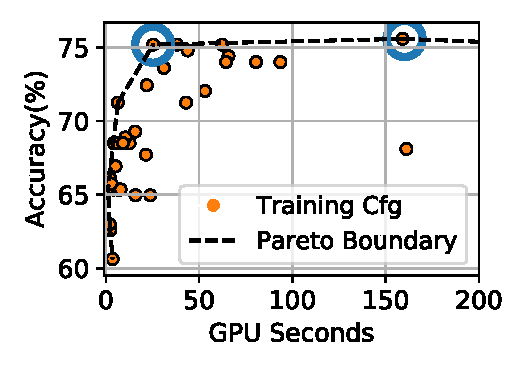
\includegraphics[width=\linewidth]{ekya/figures/motivation/AccuracyResourceProfile/jena.pdf}
    \caption{\small Resource-accuracy}
    \label{fig:darmstadt-profile}
  \end{subfigure}  
  \caption{\bf\small Measuring retraining configurations. % with the Cityscapes dataset \cite{cityscapes}.
  GPU seconds refers to the duration taken for retraining with $100\%$ GPU allocation. (a) varies two example hyperparameters, keeping others constant. Note the Pareto boundary of configurations in (b); for every non-Pareto configuration, there is at least one Pareto configuration that is better than it in {\em both} accuracy and GPU cost. }
  \label{fig:resource-profiles}
\end{figure}


\subsection{Configuration diversity of retraining and inference}
\label{subsec:profiles}

%\ion{Actually, I think the last two subsections are part of the motivation, no?} 
\noindent{\bf Tradeoffs in retraining configurations.} The hyperparameters for retraining, or ``retraining configurations'', influence the resource demands and accuracy. %of the retrained model. 
Retraining fewer layers of the DNN (or, ``freezing'' more layers) consumes lesser GPU resources, as does training on fewer data samples, but they also produce a model with lower accuracy; Figure \ref{fig:hyparam-zoom}. %but yielding the maximum possible performance from the model may require training for a longer duration.

Figure \ref{fig:darmstadt-profile} illustrates the resource-accuracy trade-offs for an edge DNN (ResNet18) with various hyperparameters: number of training epochs, batch sizes, number of neurons in the last layer, number of frozen layers, and fraction of training data. We make two observations.
%We experiment with the following hyperparameters to retrain the ResNet18 classifier: number of epochs to train for, batch size, number of neurons in the last layer, number of layers to retrain, and the fraction of data between retraining windows to be used for retraining. We refer to every combination of these hyperparameter values as a {\em configuration}. Figure \ref{fig:resource-profiles} shows the spread among the hyperparameter configurations in their GPU resource usage and the accuracy of the retrained model.  
First, there is a wide spread in the resource usage (measured in GPU seconds), by upto a factor of $200\times$. 
%Some hyperparameter configurations lead to high accuracy but are expensive (top right of Figure \ref{fig:darmstadt-profile}), while some are cheap but lead to lower accuracy (bottom left of Figure \ref{fig:darmstadt-profile}). %Together, they form the Pareto boundary of configurations (\gaa{as marked}). 
Second, higher resource usage does not always yield higher accuracy. For the two configurations circled in Figure \ref{fig:darmstadt-profile}, their GPU demands vary by $6\times$ even though their accuracies are the same ($\sim 76\%$). Thus, careful selection of the configurations considerably impacts the resource efficiency.
% Connect this expt to 3b. Ideal - check if the pair of video-streams in 3b is similar/distinct.
\revtext{Moreover, the accuracy spread across configurations is dependent on the extent of data-drift. Retraining on visually similar data with little drift results in a narrower spread. % in accuracies.% across configurations.
}
%, To verify this, we retrained the same set of hyperparameters from Figure \ref{fig:darmstadt-profile} on a visually similar video segment as the test video segment (same time-of-day and city). Since the visual similarity results in a lower data-drift, the spread of accuracy values after retraining of the compressed models was much smaller - 6.2\%, compared to \fillme\% in Figure \ref{fig:darmstadt-profile}.}
With the changing characteristics of videos, it is challenging to efficiently obtain the resource-accuracy profiles for retraining.

% As the data drifts, if data is much more visually similar like the training configurations, the spread in accuracy is narrower for configurations


%{\em Changing profiles over time.} \romil{Talk about changing hyperparameter ordering.} \romil{Show that the profiles on the pareto boundary are predictable (or similar).}  % Changing profiles are fine as long as they are predictable.


\newcommand{\scell}[2][l]{%
  \begin{tabular}[#1]{@{}c@{}}#2\end{tabular}}
  
\begin{table}[t]
\footnotesize\addtolength{\tabcolsep}{-3pt}
\begin{tabular}{l cc cc}
\toprule
\multirow{2}{*}{\bf Configuration} & \multicolumn{2}{c}{\bf Retraining Window 1} & \multicolumn{2}{c}{\bf Retraining Window 2} \\
\cmidrule(lr){2-3} \cmidrule(lr){4-5}
& \scell{\bf End\\ \bf Accuracy} & \scell{\bf GPU\\ \bf seconds} & \scell{\bf End\\ \bf Accuracy} & \scell{\bf GPU\\\bf seconds} \\ \midrule
Video A Cfg1A       & 75    & 85    & 95    & 90      \\ \midrule
Video A Cfg2A (*)   & 70    & 65    & 90    & 40     \\ \midrule
Video B Cfg1B       & 90    & 80    & 98    & 80       \\ \midrule
Video B Cfg2B (*)   & 85    & 50    & 90    & 70\\ 
\bottomrule
\end{tabular}
\caption{\label{tab:schedmot-hypparams}\small\bf Hyperparameter configurations for retraining jobs in Figure \ref{fig:schedmot}'s example. At the start of retraining window 1, camera A's inference model has an accuracy of 65\% and camera B's inference model has an accuracy of 50\%. Asterisk (*) denotes the configurations picked in Figures \ref{fig:schedmot-res-prioritization} and \ref{fig:schedmot-prioritization}.
%\romil{FIX: The GPU time cost between retraining windows cannot be different. The cost for the configs also be the same across videos. }
% \ion{Is 20\% a realistic accuracy? I mean at this accuracy the system is quite useless, no?}
}
\end{table}

% Scheduler motivation figure
\begin{figure}[t]
  \centering
    \begin{subfigure}[t]{0.47\columnwidth}
    \centering
    %\hspace*{0.02in}
    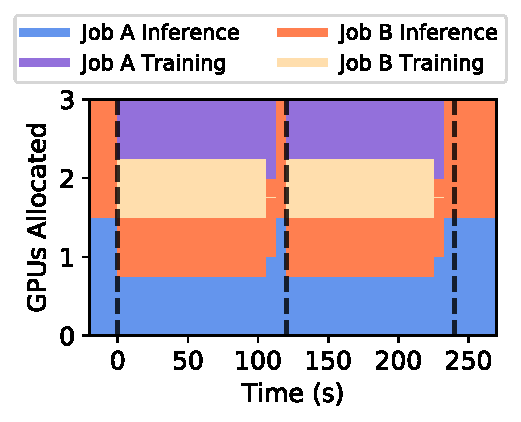
\includegraphics[width=\linewidth]{ekya/figures/motivation/Scheduler/schedmot_res_eventual_best_cfgs.pdf}
    \caption{\small Uniform scheduler}
    \label{fig:schedmot-res-naive}
  \end{subfigure}  
%  ~~
%  \begin{subfigure}[t]{0.3\linewidth}
%    \centering
%    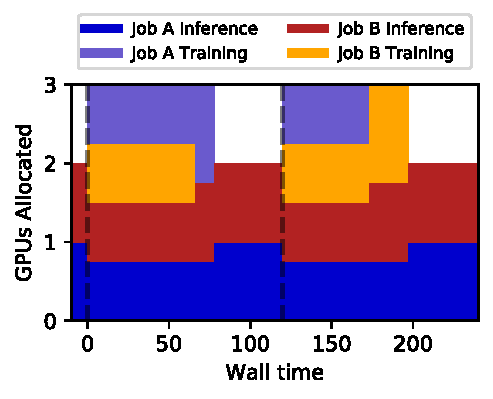
\includegraphics[width=\linewidth]{ekya/figures/motivation/Scheduler/schedmot_res_optimal_cfgs.pdf}
%    \caption{\small Optimal cfgs for retraining window}
%    \label{fig:schedmot-res-optimalcfg}
%  \end{subfigure}
  ~~
  \begin{subfigure}[t]{0.47\columnwidth}
    \centering
    %\hspace*{0.05in}
    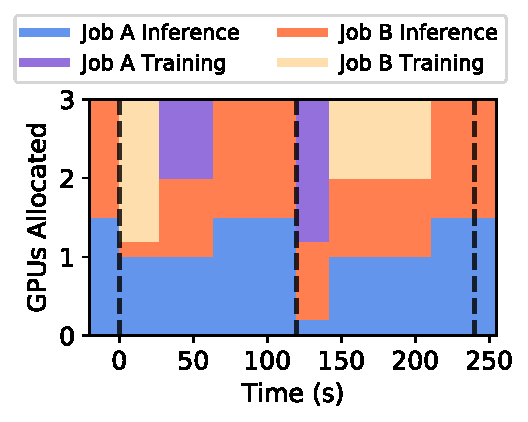
\includegraphics[width=\linewidth]{ekya/figures/motivation/Scheduler/schedmot_res_prioritization_and_optimal_cfgs.pdf}
    \caption{\small Accuracy-optimal sched.}
    \label{fig:schedmot-res-prioritization}
  \end{subfigure}
      ~~\\
  \begin{subfigure}[t]{0.47\columnwidth}
    \centering
    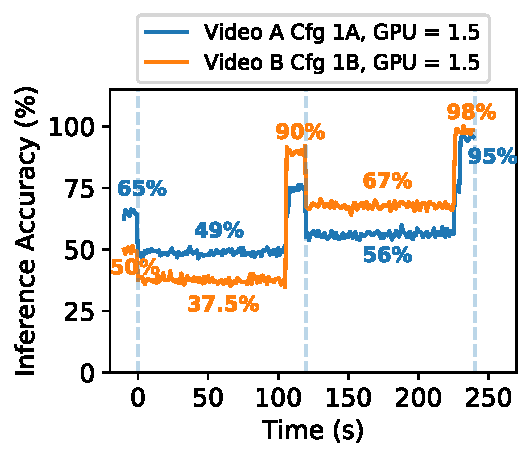
\includegraphics[width=\linewidth]{ekya/figures/motivation/Scheduler/schedmot_multiwindow_eventual_best_cfgs.pdf}
    \caption{\small Uniform scheduler}
    \label{fig:schedmot-naive}
  \end{subfigure}  
%  ~~
%  \begin{subfigure}[t]{0.3\linewidth}
%    \centering
%    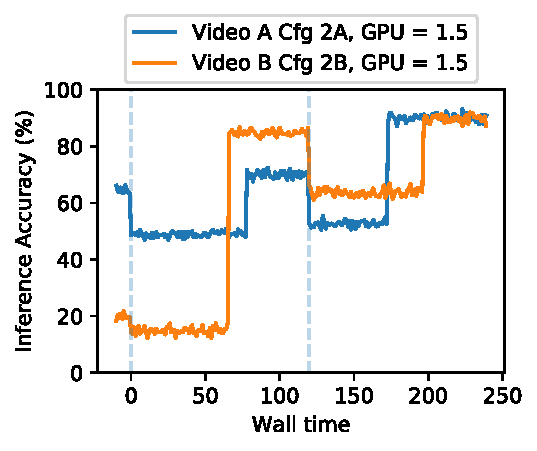
\includegraphics[width=\linewidth]{ekya/figures/motivation/Scheduler/schedmot_multiwindow_optimal_cfgs.pdf}
%    \caption{\small Optimal cfgs for retraining window}
%    \label{fig:schedmot-optimalcfg}
%  \end{subfigure}
  ~~
  \begin{subfigure}[t]{0.47\columnwidth}
    \centering
    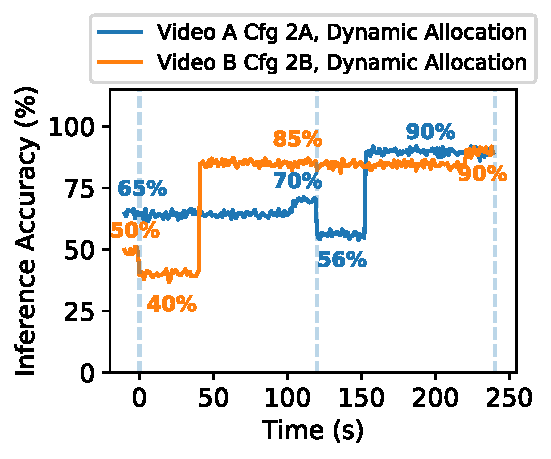
\includegraphics[width=\linewidth]{ekya/figures/motivation/Scheduler/schedmot_multiwindow_prioritization_and_optimal_cfgs.pdf}
    \caption{\small Accuracy-optimal sched.}
    \label{fig:schedmot-prioritization}
  \end{subfigure}
  ~~
  \caption{\bf\small Resource allocations (top) and inference accuracies (bottom) over time for two retraining windows (each of $120$s). The left figures show a uniform scheduler which evenly splits the $3$ GPUs, and picks configurations resulting in the most accurate models. The right figures show the accuracy-optimized scheduler that prioritizes resources and optimizes for inference accuracy averaged over the retraining window ($73\%$ compared to the uniform scheduler's $56\%$). The accuracy-optimized scheduler also ensures that inference accuracy never drops below a minimum (set to $40\%$ in this example, denoted as $a_\text{MIN}$). %\ga{Needs better colors.} \ga{Visually align x-axes in Figures 5a, 5c and Figures 5b, 5d.}
  %\ion{The problem I have with this example is that the "optimal" solution in (d) gets lower minima. It is just not clear to me why a better average but a lower min is necessary better than a lower average but a higher min.} 
  %\romil{Make this easier to read by adding text annotations to accuracy when it changes }
  %Resource allocation maps for toy retraining schedules in Figure \ref{fig:schedmot}. (\ref{fig:schedmot-naive}) and (\ref{fig:schedmot-res-optimalcfg}) run a fair scheduler which evenly splits resources between the two cameras. (\ref{fig:schedmot-res-prioritization}) deprioritizes Camera B's inference task due because of its low accuracy, and instead focuses resources on retraining it. On the other hand, Camera A's inference job is already at an high accuracy, thus it deprioritizes it's retraining job until Camera B is retrained.
  }
  \label{fig:schedmot}
\end{figure}


\noindent{\bf Tradeoffs in inference configurations.} %As described in \S\ref{subsec:edge}, inference operations using the DNNs on the live video streams is a key workload on edge servers. 
Inference pipelines also allow for flexibility in their resource demands at the cost of accuracy through configurations to downsize and sample frames \cite{rocket-github}. \revtext{Reducing the resource allocation to inference pipelines increases the processing latency per frame, which then calls for sub-sampling the incoming frames to match the processing rate, that in turn reduces inference accuracy \cite{videostorm}.} 
Prior work has made dramatic advancements in %configurations to control the resource usage of inference operations by downsizing frames to lower resolutions and sampling of frames, as well as 
profilers that efficiently obtain the resource-accuracy relationship for {\em inference configurations} \cite{chameleon}. We use these efficient inference profilers in our solution, and also to ensure that the inference pipelines keep up with analyzing the live video streams. % with their currently allocated resources. %We use these profilers in our solution to ensure that inference pipelines continue to keep up with analyzing the live video streams with their currently allocated resources.% even as they produce outputs of lower accuracy during the retraining.
%- \romil{Talk about the phenomenon of decrease in accuracy when inference is resource-starved. Any sources? Chameleon?}


%Since each model has multiple resource-accuracy configurations to pick from (\cref{fig:resource-profiles}), the scheduler must be careful while doing this in a time-bound setting. A naive approach would be to pick the hyperparameters which yield the best accuracy at completion, but the time-sensitive nature of retraining jobs requires the scheduler to also consider the resource-cost of each model.



%\subsection{The Inference Accuracy-over-time Metric.}
%While retraining improves inference accuracy at completion, but also reduces the inference accuracy while it is running because inference resources are diverted to retraining. To capture this tradeoff, we use the inference accuracy over time metric, which is defined as the mean accuracy of the inference job over a retraining window.
%\romil{Still need to explain WHY this metric and what's a retraining window.}


% Hyperparameter table


\subsection{Illustrative scheduling example}
\label{subsec:motivation-sched-example}


We use an example with $3$ GPUs and two video streams, A and B, to show the considerations in scheduling inference and retraining tasks jointly.
Each retraining uses data samples accumulated since the {\em beginning of} the last retraining (referred to as the ``retraining window'').\footnote{Continuous learning targets retraining windows of tens of seconds to few minutes \cite{distribution-20, mullapudi2019}. We use 120 seconds in this example. Our solution is robust to and works with any given window duration for its decisions (See \S{\ref{subsec:eval-understanding}}).} % and we experiment with different durations in \S\ref{sec:evaluation}.} 
%A retraining window consists of model retraining, inference during the retraining with the old model, and inference after the retraining with the retrained model.
% setup and profiles
To simplify the example, we assume the scheduler has knowledge of the resource-accuracy profiles, but these are expensive to get in practice (we describe our efficient solution for profiling in \S\ref{subsec:profiling}).
Table \ref{tab:schedmot-hypparams} shows the retraining configurations ({\small Cfg1A, Cfg2A, Cgf1B, and Cgf2B}), their respective accuracies after the retraining, and GPU cost.
The scheduler is responsible for selecting configurations and allocating resources for inference and retraining jobs.
%Note that these values vary significantly in different windows because of data drift.
%The retraining jobs for the two video streams, A and B, have two hyperparameter configurations each ({\small Cfg1A, Cfg2A, and Cgf1B, Cgf2B}), with their respective values of accuracy after the retraining and GPU cost. Note the difference in accuracy values of the same configurations between the two retraining windows. Further, there is also considerable difference among the configurations in their GPU costs for retraining, even when their accuracies are similar (e.g., {\small Cfg2A} and {\small Cfg2B} in the second retraining window).% Finally, as we see in the second retraining window, even while camera A's end accuracies (after retraining with Cfg2) is comparable to camera B's accuracies, the latter's current (starting) accuracies are far lower. 





% retraining window, option (a), inference downgrading
%At the start of each retraining window (whose duration is $120$s in our example), resources are allocated to the retraining, even while the inferences continue to execute. The scheduler is also responsible for selecting their configurations (\S\ref{subsec:profiles}). %The choice of configurations provides flexibility in their resource demands. %\ga{Can we stagger the retraining jobs?} 


%Figure \ref{fig:schedmot} shows the effect of resource allocation on the {\em inference} accuracies of the two camera streams --  before the retraining, during the retraining, and after the retraining. The example covers two retraining windows, the choice of configurations for the two video streams, and the resource allocations for retraining and inference (Figure \ref{fig:schedmot-res}).

% fair scheduler
%\noindent{\bf Fair scheduling:} A strawman solution for resource allocation is {\em fair} scheduling \cite{fair-1, fair-2, videostorm}. The fair scheduler evenly splits the GPUs between video streams, and each stream evenly partitions its allocated GPUs for retraining and inference tasks; see Figure \ref{fig:schedmot-res-naive}. The fair scheduler picks those configurations for retraining whose retrained model has the highest accuracy ({\small Cfg1A, Cfg1B} in Table \ref{tab:schedmot-hypparams} for both windows).
\noindent{\bf {\Fair} scheduling:} Building upon prior work in cluster schedulers \cite{fair-1, fair-2} and video analytics systems \cite{videostorm}, a baseline solution for resource allocation evenly splits the GPUs between video streams, and each stream evenly partitions its allocated GPUs for retraining and inference tasks; see Figure \ref{fig:schedmot-res-naive}. Just like model training systems \cite{vizier,hyperband,pbt}, the baseline always picks the configuration for retraining that results in the highest accuracy ({\small Cfg1A, Cfg1B} for both windows).


Figure \ref{fig:schedmot-naive} shows the {\em inference} accuracies of the two live streams.
We see that when the retraining tasks take resources away from the inference tasks, the inference accuracy drops significantly ({$65\%$} $\rightarrow$ {$49\%$} for video A and {$50\%$} $\rightarrow$ {$37.5\%$} for video B in Window 1).
%--  before the retraining, during the retraining, and after the retraining -- on two retraining windows. 
%The inference jobs themselves are given lesser resources during the retraining and hence run at configurations with lower accuracy (e.g., by skipping frames). 
%The inference accuracies during the first retraining window (Figure \ref{fig:schedmot-naive}) dropped from {$65\%$} $\rightarrow$ {$49\%$} for video A and {$50\%$} $\rightarrow$ {$37.5\%$} for video B, and a similar drop in the second window. % , there is little time to use the model for inference before the next retraining window. 
%While the retrainings produced a model with higher accuracy, they also took a long time (due to high GPU costs) during which the inference accuracy was lower. 
While the inference accuracy increases \emph{after} retraining, it leaves too little time in the window to reap the benefit of retraining. 
%Averaged over the first retraining window, video A's and B's inference accuracies end up being $54\%$ and $57\%$, even though the configurations themselves ({\small Cfg1A, Cfg1B}) resulted in retrained models with much higher accuracies of $75\%$ and $90\%$ (Table \ref{tab:schedmot-hypparams}). 
Averaged across both retraining windows, the inference accuracy across the two video streams is only $56\%$ because the gains due to the improved accuracy of the retrained model are undercut by the time taken for retraining (during which inference accuracy suffered).
%As a result, this schedule results in a low mean inference accuracy of 51.82\% when measured over the entire duration of the retraining window (\gaa{120s} in our example).
%\ys{In Fig 4a, how do we ``fairly'' allocate resources after job B training finishes? Maybe we should plot the figures across two columns and vertically align a/c and b/d. }









%\noindent{\bf Retraining-aware fair scheduling:} An alternative to the above fair scheduler is picking hyperparameter configurations with lower GPU demands that train faster ({\small Cfg2A} and {\small Cfg2B}; Table \ref{tab:schedmot-hypparams}), and thus allows for inference on the retrained model (with higher accuracy) for a longer duration in the retraining window (see Figure \ref{fig:schedmot-optimalcfg}). This scheme results in the average inference accuracy across the two retraining windows of 62.4\% for the two video streams. However, this scheme still equally partitions resources between the two video streams, allocating 1.5 GPU to each, and further equally allocates it's share to inference and retraining tasks (Figure \ref{fig:schedmot-res-optimalcfg}).  %This is a suboptimal resource allocation, as demonstrated in 

\noindent{\bf Accuracy-optimized scheduling:} %Figures \ref{fig:schedmot-res-prioritization} and \ref{fig:schedmot-prioritization} illustrate an accuracy-optimized scheduler, which takes a holistic view on the multi-dimensional tradeoffs in selecting hyperpareamter configurations and allocating resources.
Figures \ref{fig:schedmot-res-prioritization} and \ref{fig:schedmot-prioritization} illustrate an accuracy-optimized scheduler, which by taking a holistic view on the multi-dimensional tradeoffs, provides an an average inference accuracy of $73\%$. In fact, to match the accuracies, the above {\fair} scheduler would require nearly twice the GPUs (i.e., $6$ GPUs instead of $3$ GPUs). 

This scheduler makes three key improvements. First, the scheduler selects the hyperparameter configurations based on their accuracy improvements \emph{relative} to their GPU cost. It selects lower accuracy options ({\small Cfg2A/Cfg2B}) instead of the higher accuracy ones ({\small Cfg1A/Cfg1B}) because these configurations are substantially cheaper (Table \ref{tab:schedmot-hypparams}). 
Second, the scheduler \emph{prioritizes} retraining tasks that yield higher accuracy, so there is more time to reap the benefit from retraining. For example, the scheduler prioritizes B's retraining in Window 1 as its inference accuracy after retraining increases by $35\%$ (compared to $5\%$ for video A).
Third, the scheduler controls the accuracy drops during retraining by balancing the retraining time and the resources taken away from inference. %\footnote{The techniques in our scheduler apply to other optimization metrics too, like max-min of accuracy. Evaluating other metrics is left to future work.}

%The scheduler ensures a minimum inference accuracy (40\% in this example) at all times.


%($1$) Hyperparameter configurations are chosen based on the {\em improvement in accuracy} due to the retraining {\em relative to its GPU cost}. In the first retraining window, {\small Cfg2} is chosen for video B even though its accuracy is lower than {\small Cfg1}'s accuracy, because of {\small Cfg2}'s substantially cheaper resource cost (50 GPU-seconds as opposed to 80; Table \ref{tab:schedmot-hypparams}). 

%\noindent{Resource} allocation is also based on the improvement in accuracy and resource costs. In Figure \ref{fig:schedmot-res-prioritization}, video B's retraining is prioritized in the first retraining window because its accuracy is expected to go up from {$50\%$} to $85\%$ while video A's accuracy improves from {$65\%$} to only $70\%$; see Figure \ref{fig:schedmot-prioritization}. Further, the cost of retraining B ($50$ GPU-seconds) is lower than retraining A ($65$ GPU-seconds). 
%However, camera A's retraining is prioritized in the next window of Figure \ref{fig:schedmot-res-prioritization}.
%Likewise, in the second retraining window, camera A's accuracy has a much higher increase (70\% to 90\%), and thus its training is prioritized (note that camera B's retraining is prioritized in first retraining window). 

%($2$) Resource allocations are {\em jointly decided for inference and training}. In the first retraining window of Figure \ref{fig:schedmot-res-prioritization}, while video B's models are being retrained, resources are taken away from video B's inference (but not from inference of video A). Likewise with video A in the second  window. 

%($3$) Resource allocations and configuration selections optimize the {\em inference accuracy over the retraining window}, i.e., compensating for the reduced inference accuracy during the retraining with the higher accuracy model after the retraining. 

%Taking a holistic view on configuration selection and resource allocation leads to an average inference accuracy of $73\%$ across the two videos and two retraining windows, which is far higher than the earlier {\fair} scheduler ($56\%$). In fact, to match the accuracies, the {\fair} scheduling would require nearly twice the GPU resources (i.e., $6$ GPUs in our example, instead of the currently provisioned $3$ GPUs). 
%We also evaluated a variant of the accuracy-optimized scheduler that chooses configurations as per the principles above but allocates the GPU resources fairly. This lowers the average inference accuracy to $66\%$ (details omitted). Hence, it is crucial to {\em jointly select the configurations and allocate resources}.

%  Aross multiple retraining windows, show:
% \begin{itemize}
%     \item Assume linear degradation of inference
%     \item \textbf{Prioritizing one job over the other based on accuracy estimates}
%     \item \textbf{Picking different hyperparameter within a job}
%     \item \textbf{Accuracy improvement compared to fair sched}
% \end{itemize}
% Give sim examples - fair sched vs best sched

%\subsection{Challenges and Desirable properties}

%The profiles in \S\ref{subsec:profiles} and the example in \S\ref{subsec:motivation-sched-example} highlight the key desirable properties and challenges in developing our solution. ($a$) We need a resource-efficient approach to profiling the retraining jobs to obtain the accuracy of the retrained models and their resource costs, ($b$) Scheduling the resources on the edge should jointly consider both the retraining jobs as well as the inference operations on the live videos, and ($c$) The system should optimize for the accuracy of the inference operations averaged over time, instead of instantaneous values of the inference or accuracy of the retrained models alone.

